\chapter{All-sky Analysis}
  \label{sec:analysis}

    We first would like to note that ``all-sky analysis'' can be a bit misleading. The term tends to lead readers to the idea of a definitive study

    We will first introduce our all-sky analysis of the AME vs. IR emission. This approach relies on HEALPix maps smoothed to  ~1$^{\circ}$ angular resolution. We start with an all-sky AME to IR comparison, looking for global patterns among all pixels (except those within 10$^{\circ}$ of the ecliptic plane.)

\section{All-sky Pixel Domain Analysis}
  \subsection{All-sky cross correlations}
  	In order to look more closely how the the AME to IR relationship varies with wavelength, we first do a simple cross-correlation test. Figure \ref{fig:AMEvsDust_allsky_allbands} shows Spearman's $\rho$ ($r_{S}$)
    %\footnote{:<math>r_s = \rho_{\operatorname{rg}_X,\operatorname{rg}_Y} = \frac {\operatorname{cov}(\operatorname{rg}_X,\operatorname{rg}_Y)} { \sigma_{\operatorname{rg}_X} \sigma_{\operatorname{rg}_Y} }</math>}
    , for each of the 12 bands sampled.{Throughout this work we adopt $r_{s}$ as our statistical metric. Rather than the linearity of potential IR-MW relationships, we are primarily interested in the extent of monotonic relatedness.

    \subsection{Pixel mask}
      \paragraph{Zodical light}
        To keep our analysis comparable to previous works, we exclude pixels within 10$^{\circ}$ of the ecliptic plane. Even though we use the Zodi-subtracted maps (\citep{kelsall98, kondo16}), the Zodi residuals are still problematic (especially in the MIR.) Espeically at high ecliptic latitudes, the relative uncertainty of the Zodi-level is not well estimated; S/N may significantly reduced in for faint pixels, mainly for the 9 through 25~$\mu$m.

    \subsection{AME data}
       The AME data comes from the PR2 astrophysical component datasets, as described in Ch. \ref{ch:datasources}. We show the comparison for 3 different AME estimates: the two AME components ($AME_{var}$ and $AME_{fix}$) as they are provided in PR2 (intensities quoted at reference frequencies\footnote{22.8~GHz for $AME_{var}$, 41~GHz for $AME_{fix}$}. The  $AME_{fix}$ peak freq. is spatially constant at 33.5~GHz ), with $AME_{var}$ and $AME_{fix}$ calculated at each pixel's peak frequency rather than the PR2 reference freq. We do this because there is nothing physically special about the Planck reference frequencies, and because the PR2 $AME_{var}$ component intensity could vary significantly from the intensity at the peak of the fitted spinning dust template. Thirdly we show the corr-correlation matrix with a single AME metric- calculating the integrated intensity at each pixel, for both AME components, creating an $AME_{sum}$ component.



     Figure \ref{fig:AME_IR_crosscorr_allbandsg} visualizes the cross-correlation matrix for each of the IR bands. The AME does not show a strong correlation with other bands at $|l|>10$. At $|l|<10$, the FIR bands show stronger correlation. The PAH-tracing bands show a stronger correlation than bands at 18 to 60~$\mu$m, but weaker than AME vs. the FIR bands.

  \section{Spatial variaton of correlations}
    To understand how these trends may vary across the sky, we produce an all-sky maps of $r_{s}$ for AME vs. IR emission. From the NSIDE 256 input maps of AME and 4 IR wavelength maps, we produce NSIDE~8 maps of $r_{s}$. These maps are shown in Fig. \hyperref[fig:Spearman_Map_nside8_AMEtoIR]{\ref*{fig:Spearman_Map_nside8_AMEtoIR}}.

      \begin{figure*}
        \label{fig:AME_IR_crosscorr_allbandsg}
        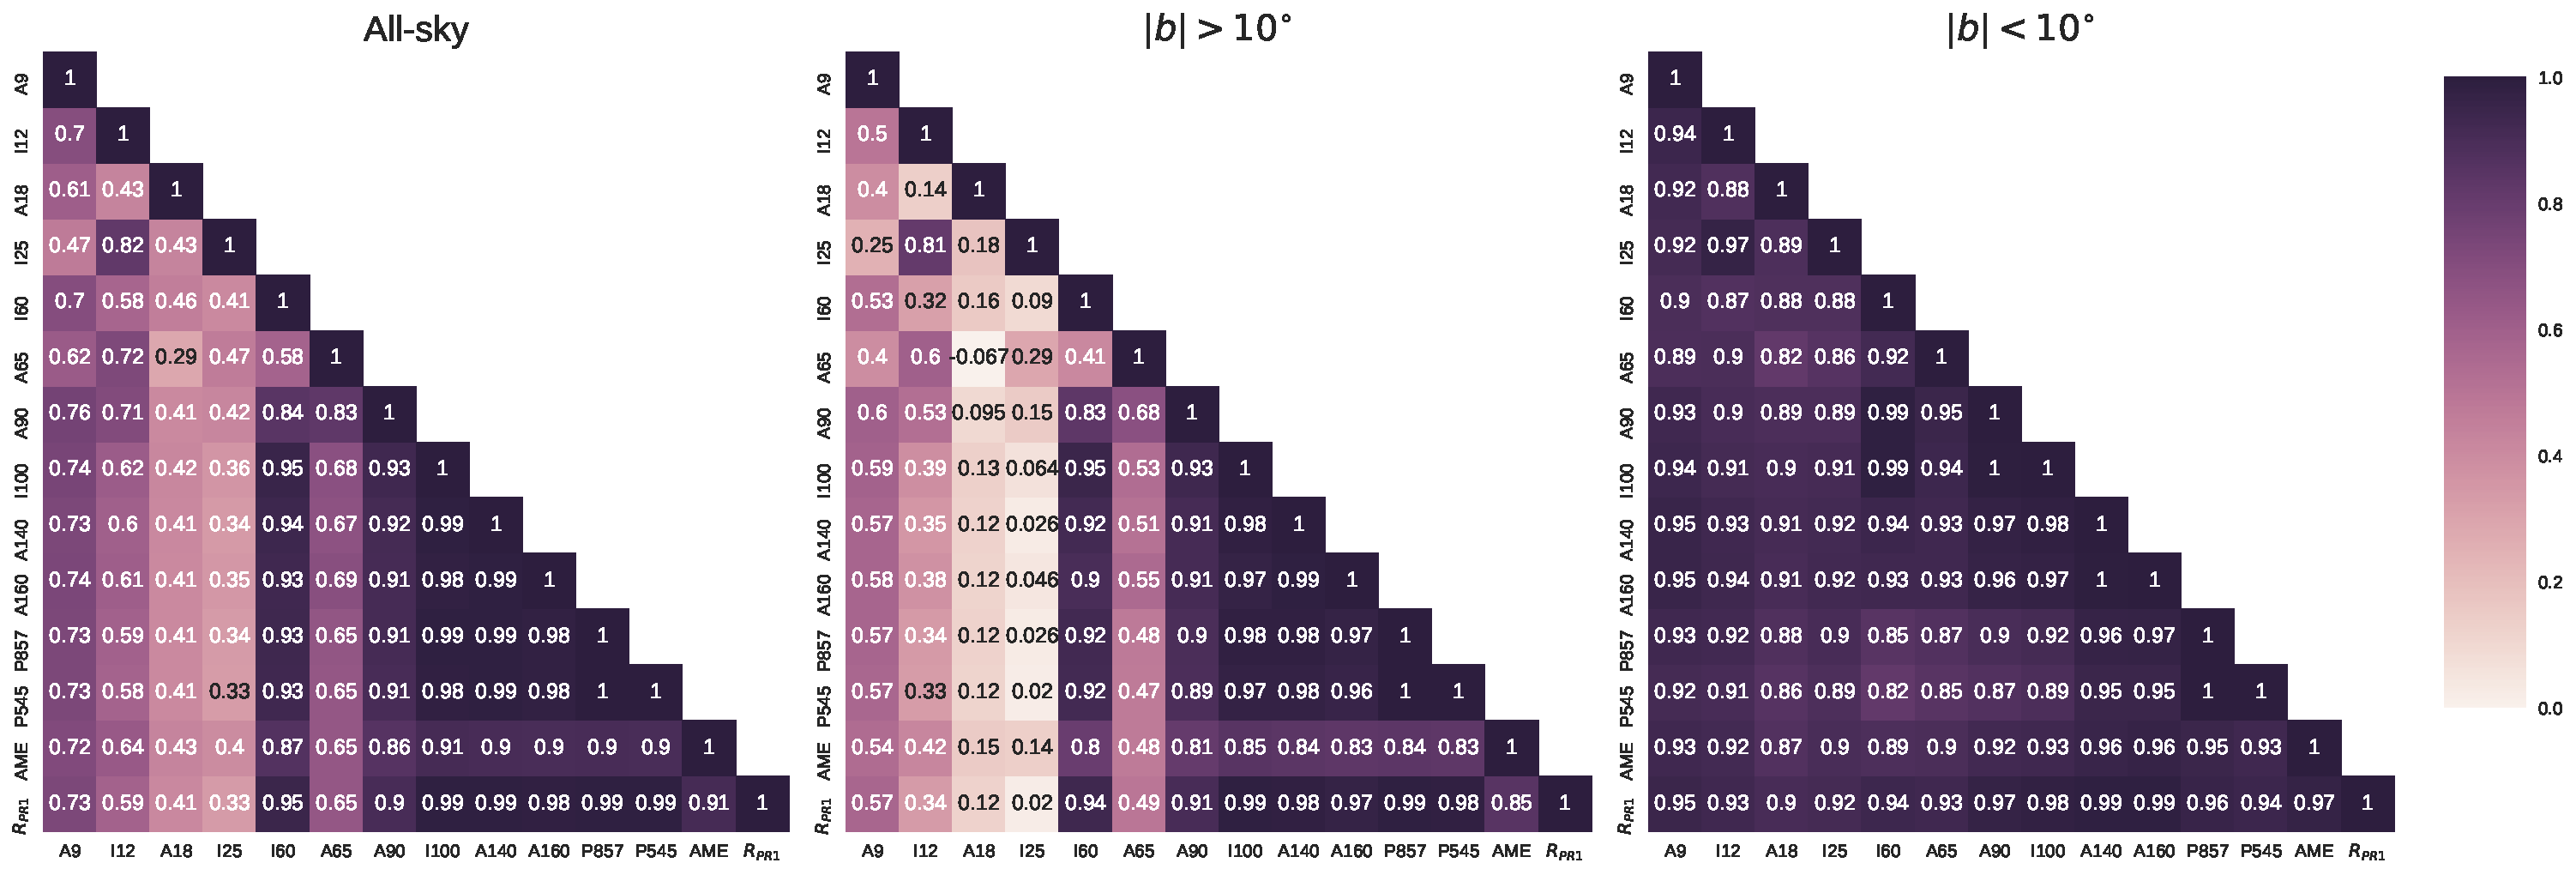
\includegraphics[width=\textwidth]{../Plots/all_bands_corr_matrix_wAME_spearman.pdf}
        \centering
        \caption{ALL-SKY cross-correlation matrix for the 18 infrared bands sampled, and the AME map. THe color-scale indicates ($r_{S}$). Results are based on the full sky (excluding pixels within 10$^{\circ}$ of the ecliptic plane).}
      \end{figure*}

      \begin{figure*}
        \label{fig:AMEvsDust_allsky_allbands}
        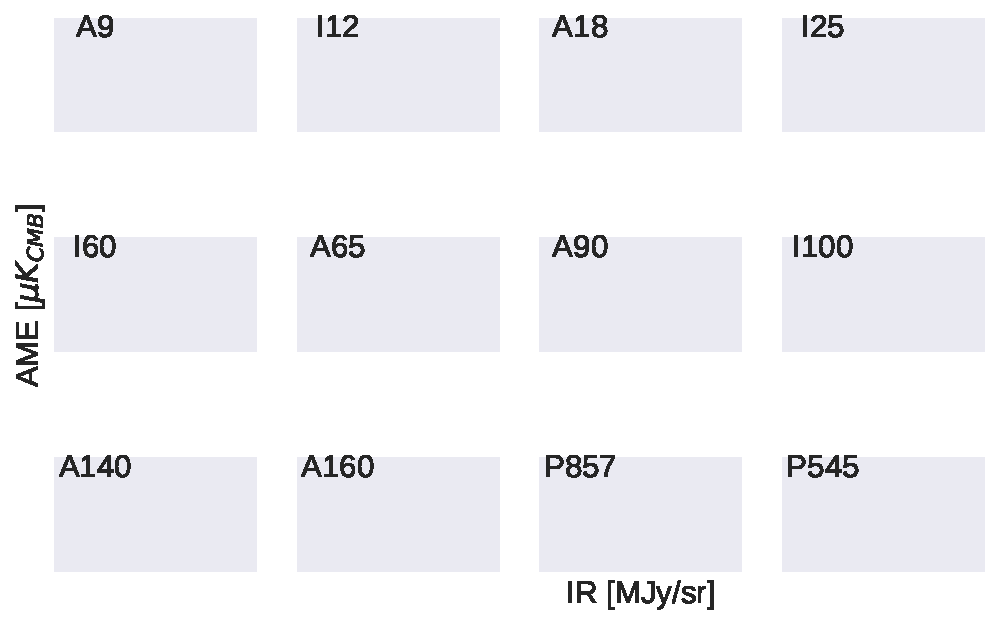
\includegraphics[width=\textwidth]{../Plots/AMEvsDust_allsky_allbands.pdf}
        \centering
        \caption{ALL-SKY kernel density estimates of 12-band infrared photometry against the PR2 AME map. Pixels within 10$^{\circ}$ of the ecliptic plane are excluded. 'A' indicates AKARI; 'D', DIRBE; 'I', IRAS, and 'P' Planck. The number after each letter indicates the band central nominal wavelength in microns (or frequency in GHz, in the case of the Planck bands.) }
      \end{figure*}

      \begin{figure*}
        \label{fig:AMEtoRvsDusttoR_allsky_allbands}
        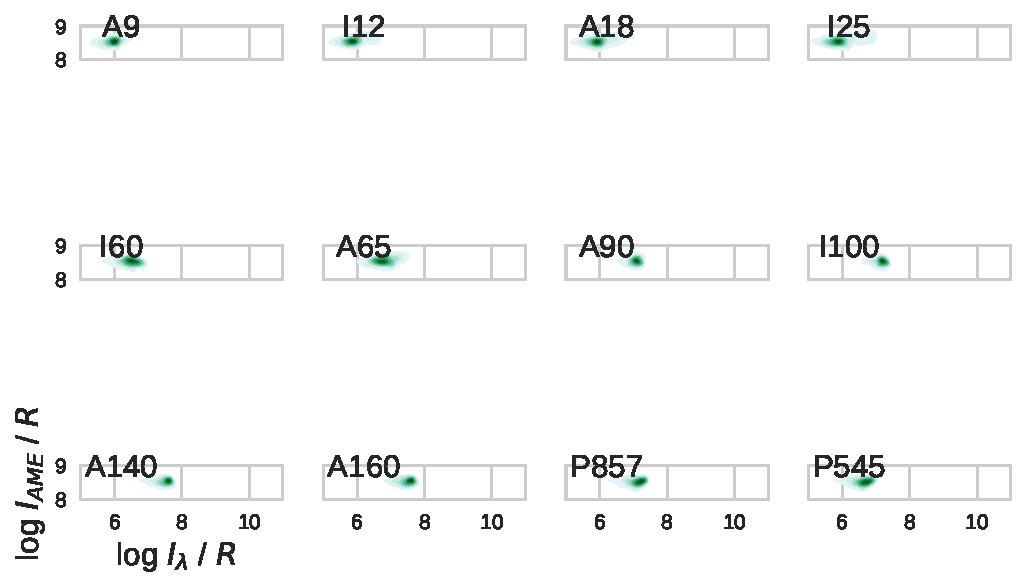
\includegraphics[width=\textwidth]{../Plots/AMEvsDust_allsky_allbands__mpsub_Rnorm_kde.pdf}
        \centering
        \caption{Similar comparison to Fig. \ref{fig:AMEvsDust_allsky_allbands}, with both the IR and the AME intensities scaled by the PR2 dust radiance ($R$) for each pixel. }
      \end{figure*}

      \begin{figure*}
        \label{fig:Spearman_Map_nside8_AMEtoIR}
        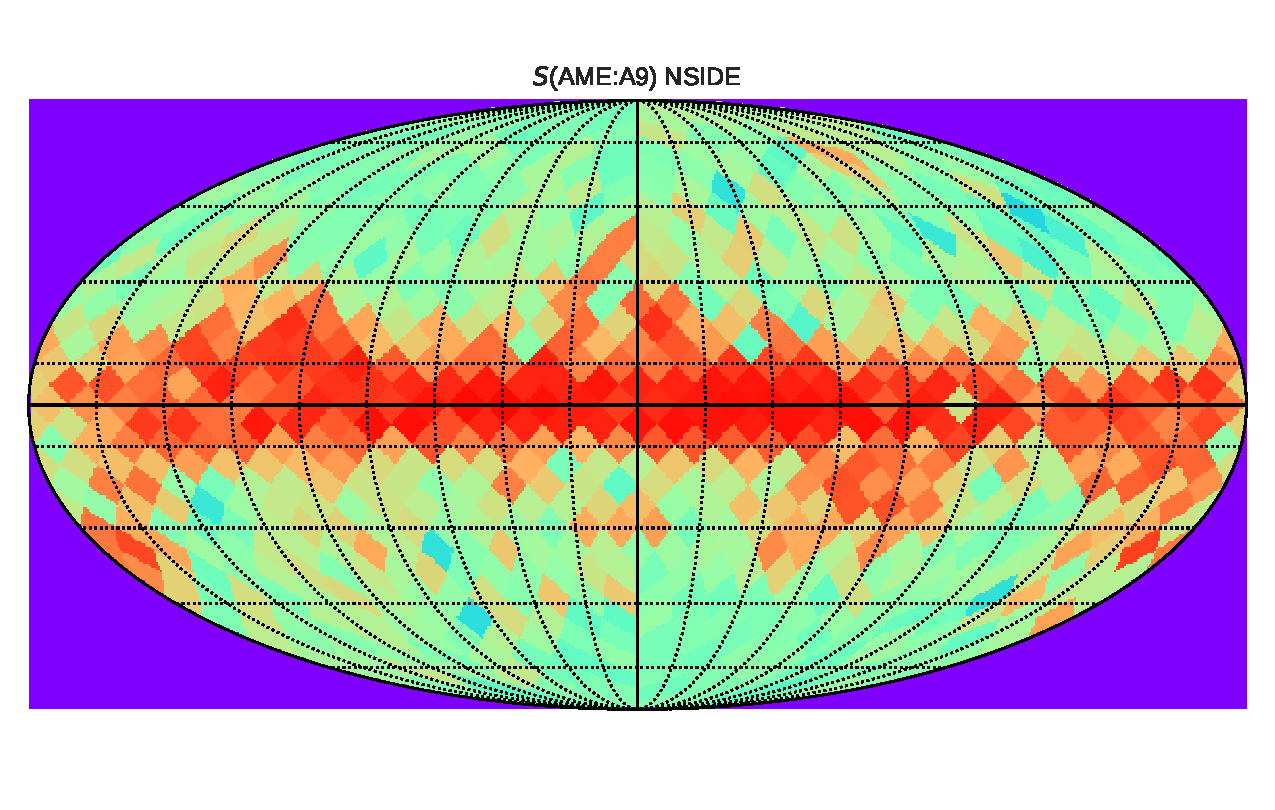
\includegraphics[width=80mm]{../Plots/Allsky_Corr/Spearman_Map_nside8_AMEtoA9.pdf}
        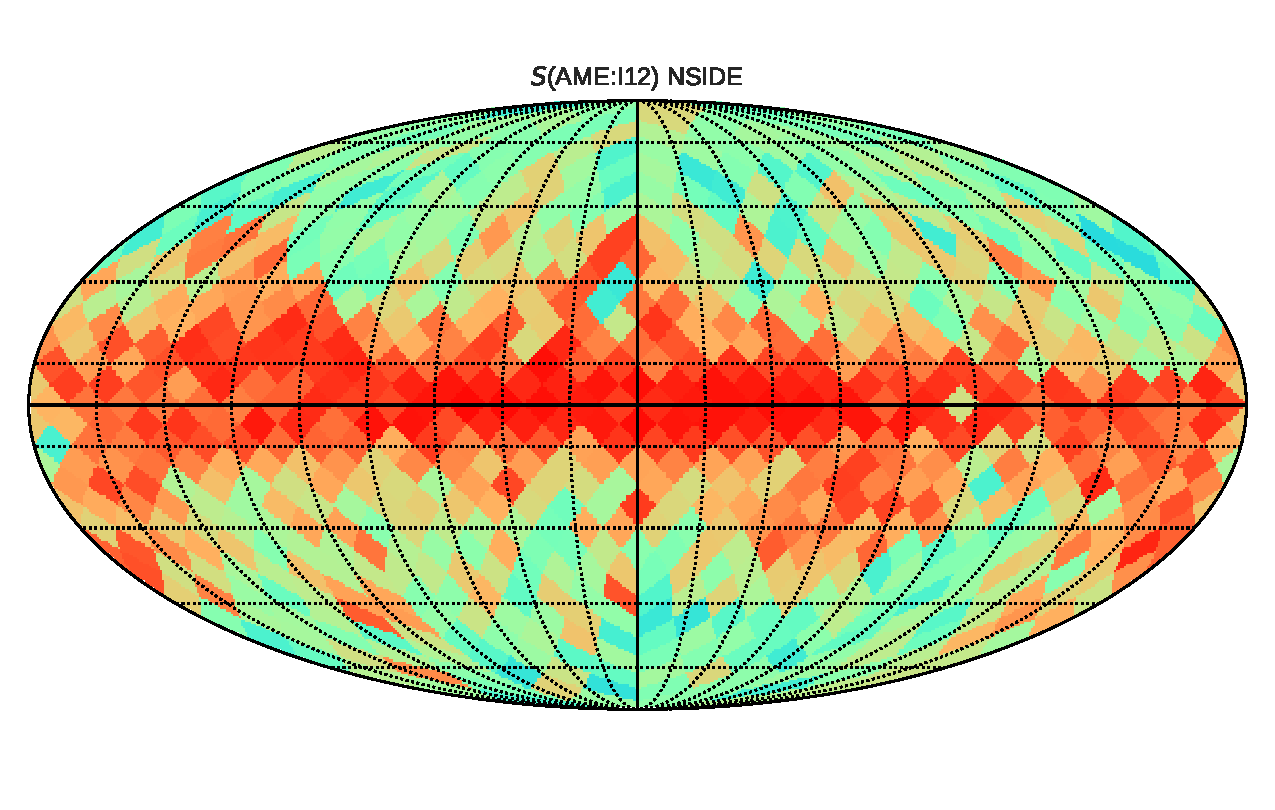
\includegraphics[width=80mm]{../Plots/Allsky_Corr/Spearman_Map_nside8_AMEtoI12.pdf}
        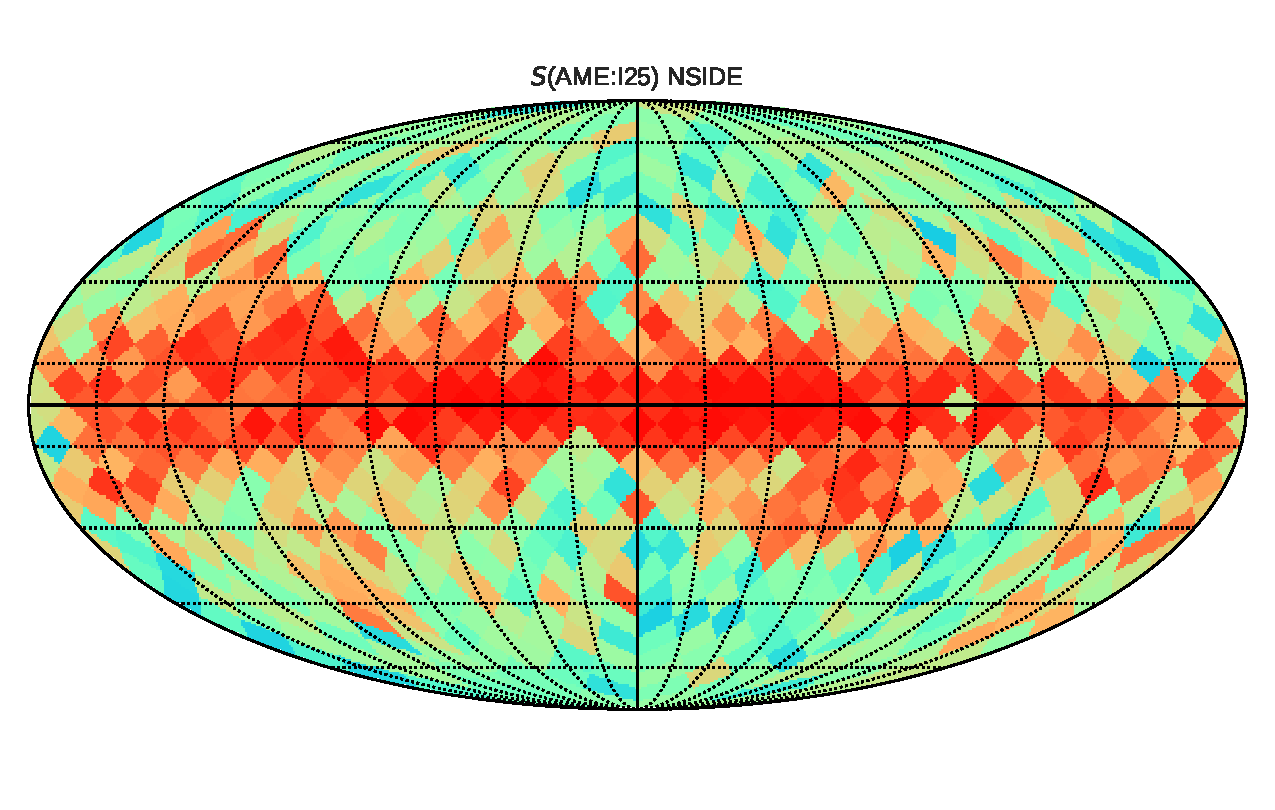
\includegraphics[width=80mm]{../Plots/Allsky_Corr/Spearman_Map_nside8_AMEtoI25.pdf}
        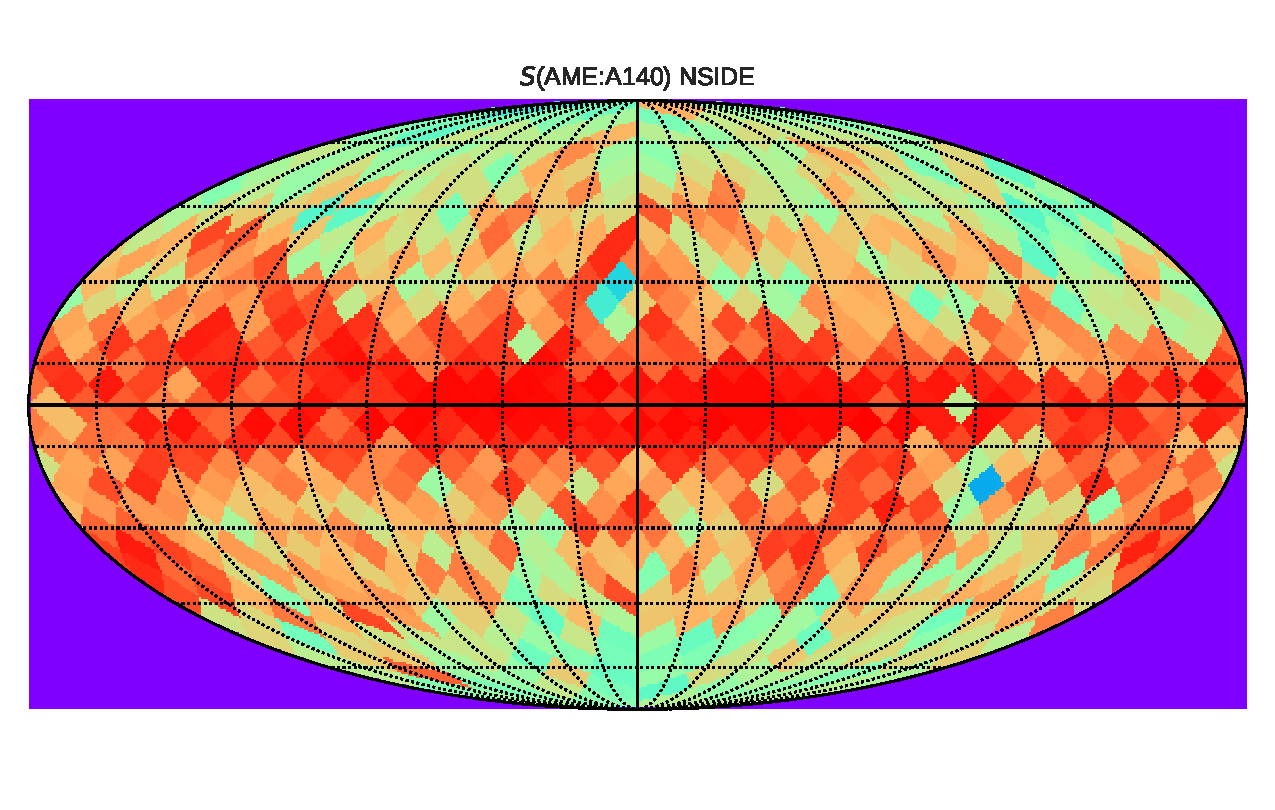
\includegraphics[width=80mm]{../Plots/Allsky_Corr/Spearman_Map_nside8_AMEtoA140.pdf}
        \centering
        \caption{Spatial map of $r_{s}$ between the AME and IR intensity for 4 bands:$9~\mu{}m$, $12~\mu{}m$, $25~\mu{}m$, and $140~\mu{}m$. $r_{s}$ is calculated for all NSIDE~256 pixels within each NSIDE~8 pixel-sized bin.}
      \end{figure*}

      \begin{figure*}
        \label{fig:Spearman_Map_nside8_AMEtoIR_radnorm}
      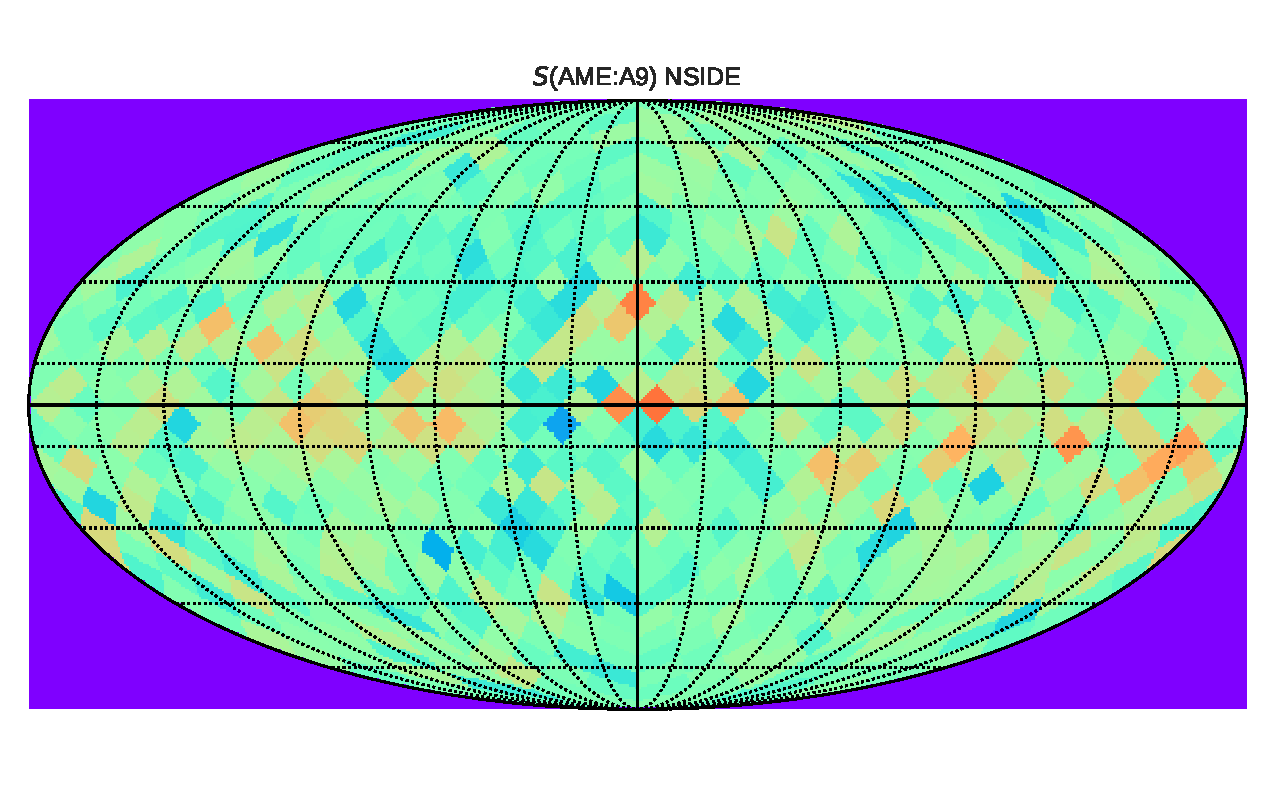
\includegraphics[width=80mm]{../Plots/Allsky_Corr/RadNorm/Spearman_Map_nside8_AMEtoA9.pdf}
      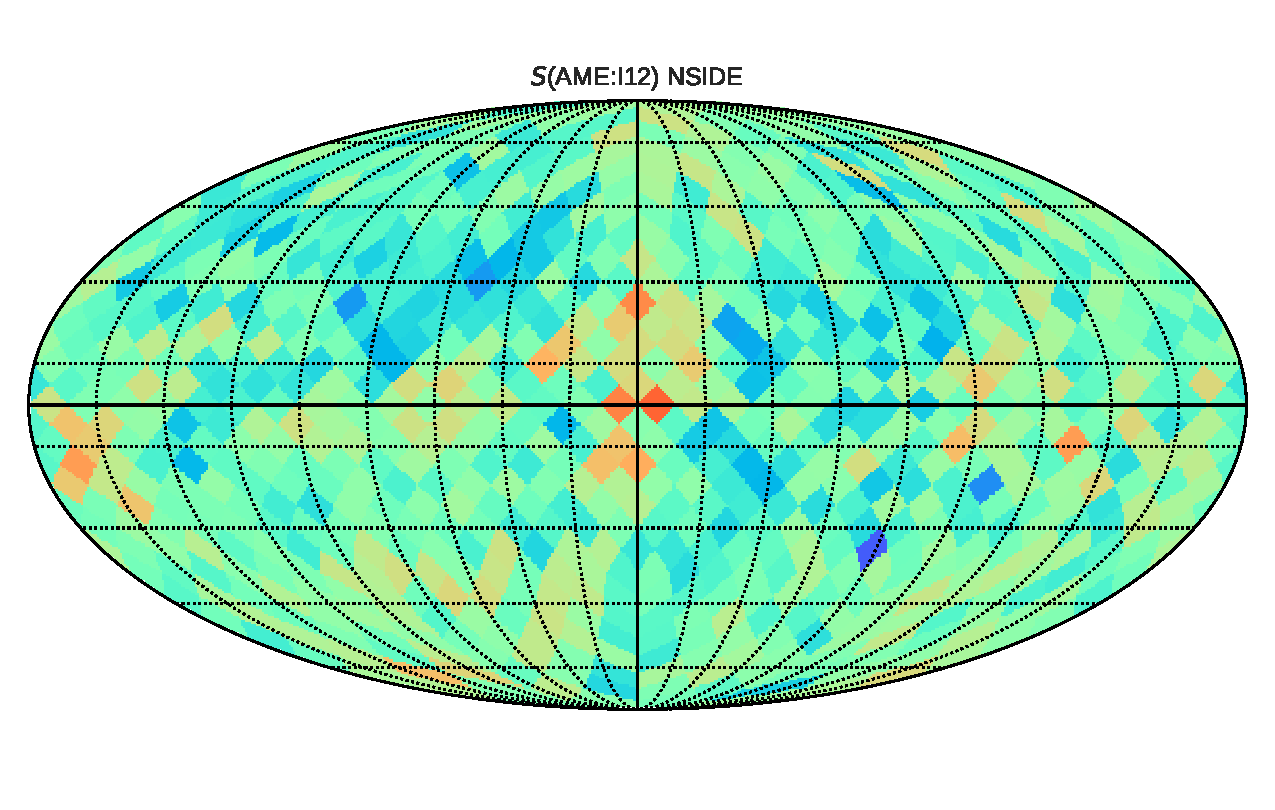
\includegraphics[width=80mm]{../Plots/Allsky_Corr/RadNorm/Spearman_Map_nside8_AMEtoI12.pdf}
      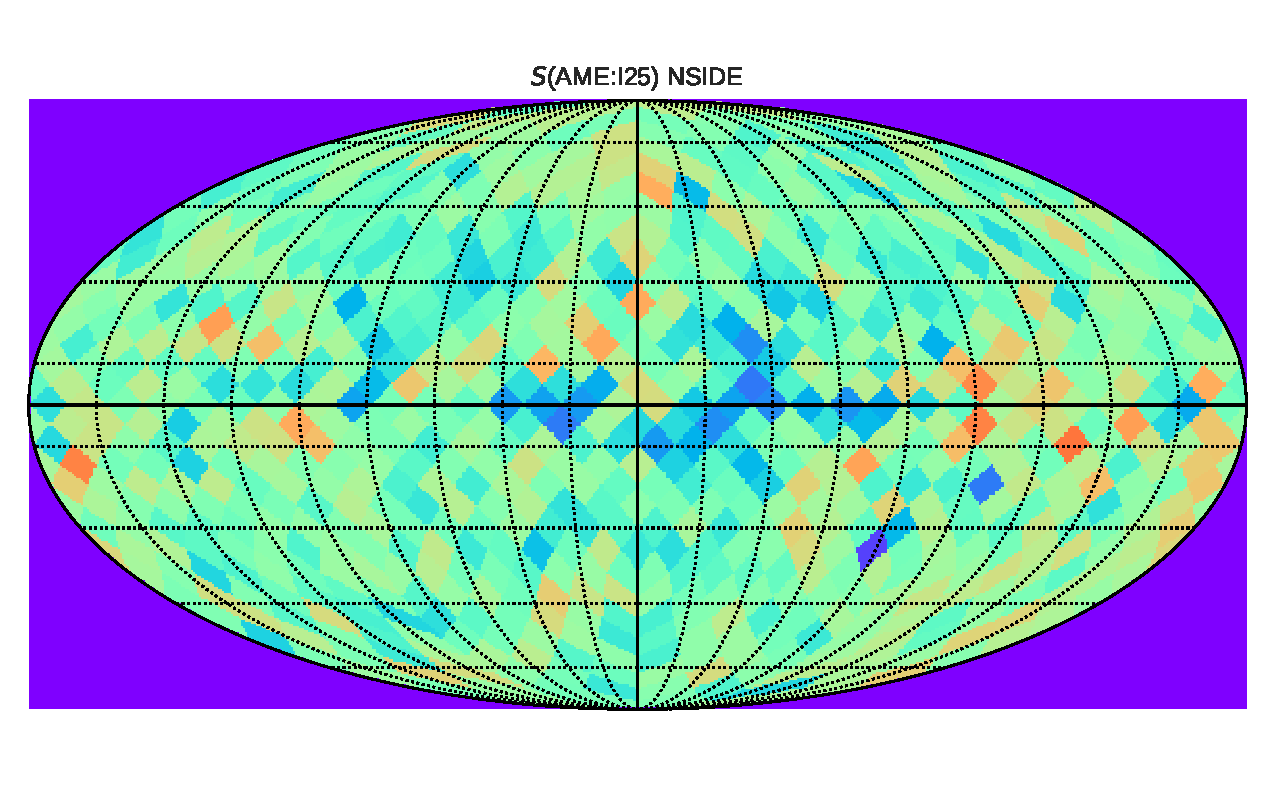
\includegraphics[width=80mm]{../Plots/Allsky_Corr/RadNorm/Spearman_Map_nside8_AMEtoI25.pdf}
      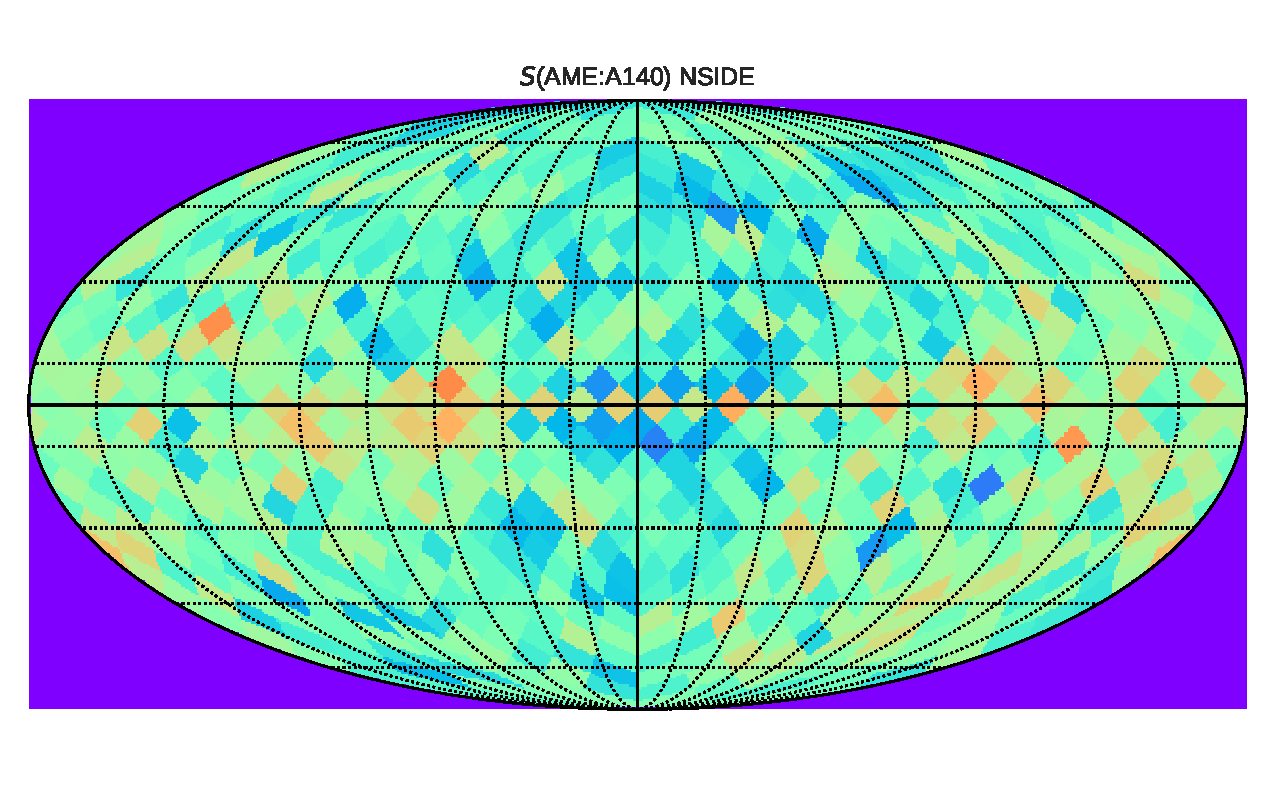
\includegraphics[width=80mm]{../Plots/Allsky_Corr/RadNorm/Spearman_Map_nside8_AMEtoA140.pdf}
      \centering
      \caption{Spatial map of $r_{s}$ between the AME and IR intensity as in Fig. \ref{fig:Spearman_Map_nside8_AMEtoIR}, but with the AME and IR maps first normalized by dust radiance $R$.}
    \end{figure*}


    \section{Discussion}
      \subsection{AME:Dust}
        As noted in Ch. \hyperref[ch:intro]{\ref*{ch:intro}}, previous studies found that the AME generally correlates at dust-related IR wavelengths \citep{ysard10b,planckXV, hensley16}. We see the same overall pattern in the present study.

         In our all-sky comparison, we find a first-order correlation between IR intensity and AME intensity, for each of the 12 wavelengths sampled. This is again consistent with the previous investigations of the AME cited above, in that the FIR emission shows the tightest correlation with the AME intensity.

         In testing for a second-order correlation, we divided the IR intensities and AME intensity by the dust radiance, and again performed the band-by-band all-sky comparison. There is evidence of a residual correlation between $I_{MIR}$ and $I_{AME}/R$. Unsurprisingly, the strong correlation between $I_{FIR}$ and $I_{AME}$ disappears when scaling by $R$, as the the FIR bands are dominated by thermal dust emission. In this case, we again find no evidence of an improved correlation for the PAH-dominated bands.

           The closeness of the correlation coefficients found here is consistent with the results of the IRAS vs. AME correlation test result from \cite{planckXV}. They found that the correlation coefficient among the 4 IRAS bands (12, 25, 60, and 100~$\mu$m) differ from one another only by about 5\%, across the whole set of 98 regions. The trend of AKARI MIR and FIR data vs. the AME does not disagree with their IRAS comparison. This work adds that bands longer than IRAS 100~$\mu$m also correlate strongly with AME, especially the two Planck/HFI bands used.

          \subsection{AME:PAH}
            Each of the bands sampled show correlation with the AME, however the FIR bands always show the strongest correlation. In fact, the correlation pattern of AME vs. each of the IR bands, very strongly resembles the correlation results of the Planck HFI bands vs. all of the other bands (Fig. \ref{fig:AME_IR_crosscorr_allbandsg}.) This is readily apparent from the pixel-density plots in Fig. \ref{fig:AMEvsDust_allsky_allbands}, wherein the FIR bands pixels show a very similar density profile vs. the AME. In attempting to factor out this first-order correlation, dividing the AME and IR intensities by the dust radiance for each pixel, we find the there is still a residual correlation between the MIR bands and the AME. The FIR bands scaled by the dust radiance, as expected, lack correlation with $I_{AME}/R$.

          \subsection{AME:$T$, $G_{0}$}
            According to spinning dust theory outlined in \cite{draine98a} and in subsequent works by \cite{ysard10a}, the AME profile and intensity will depend in part on the ISRF- but as is well-stated in \cite{hensley17a}, exactly how the ISRF will affect the AME SED is a more complicated question. Absorbed starlight photons may be able to rotationally excite the carriers, but if an enhanced ISRF leads to increased dust heating, then the increased IR emission can rotationally de-excite the carriers. However the ISRF affects not only the dust temperature but ionization of the carriers.

            \cite{hensley16} looked at the $AME$/$R$ ratio vs. $T$ and found only a slight anti-correlation of $P = -0.06$.

          \subsection{Microwave foreground component separation}

            There are known degeneracies between the foreground parameters of the COMMANDER maps (spinning-dust, and free-free, synchrotron components as described in \cite{planck15X}.) This can be demonstrated by comparing the ratio map of the PCXV intensity to thermal dust intensity.
